\begin{minipage}{\linewidth}
    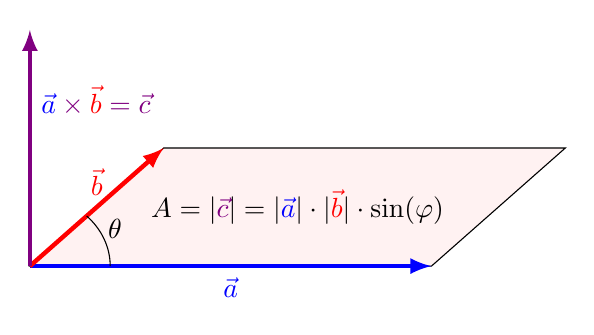
\begin{tikzpicture}[yscale=1.5, xscale=1.7, every node/.style={scale=1}]
    % Rechteck
    \draw[-,fill=white!95!red](0,0)--(3,0)--(4,1)--(1,1)--cycle;
    % Formel in der Fläche
    \node at (2,0.5) {$A = |\textcolor{violet}{\vec{c}} | = |\textcolor{blue}{\vec{a}}| \cdot |\textcolor{red}{\vec{b}}| \cdot \sin(\varphi)$};
    % a
    \draw[ultra thick,-latex,blue](0,0)--(3,0)node[midway,below]{$\vec{a}$};
    % b
    \draw[ultra thick,-latex,red](0,0)--(1,1)node[midway,above]{$\vec{b}$};
    % a x b
    \draw[ultra thick,-latex,blue!50!red](0,0)--(0,2)node[pos=0.7,right]{$\textcolor{blue}{\vec{a}} \times \textcolor{red}{\vec{b}} = \vec{c}$};
    \draw (0.6,0) arc [start angle=0,end angle=45,radius=0.6]
    node[pos=0.7,right]{$\theta$};
    \end{tikzpicture}
\end{minipage}